\documentclass{article}
\usepackage{amsmath}
\usepackage{tikz}
\usetikzlibrary{arrows.meta}

\begin{document}

\begin{figure}[h]
    \centering
    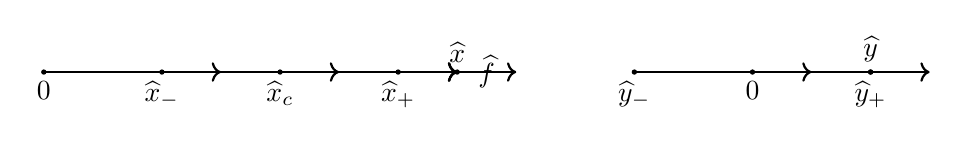
\begin{tikzpicture}[scale=1.5]
        % Draw the horizontal line with labels
        \draw[thick] (0,0) -- (4,0);
        
        % Mark the points on the left side
        \draw[fill=black] (0,0) circle (0.5pt) node[below] {$0$};
        \draw[fill=black] (1,0) circle (0.5pt) node[below] {$\widehat{x}_{-}$};
        \draw[fill=black] (2,0) circle (0.5pt) node[below] {$\widehat{x}_{c}$};
        
        % Arrows and labels for the left side
        \draw[->, thick] (1,0) -- (1.5,0);
        \draw[->, thick] (2,0) -- (2.5,0);
        \draw[->, thick] (3,0) -- (3.5,0);
        \draw[->, thick] (3,0) -- (3.5,0);
        \draw[->, thick] (3,0) -- (3.5,0);
        
        % Mark the point on the right side
        \draw[fill=black] (3,0) circle (0.5pt) node[below] {$\widehat{x}_{+}$};
        \draw[fill=black] (3.5,0) circle (0.5pt) node[above] {$\widehat{x}$};
        
        % Draw the arrow for f
        \draw[->, thick] (3.5,0) -- (4,0);
        \node at (3.75,0) {$\widehat{f}$};
        
        % Draw the horizontal line with labels on the right side
        \draw[thick] (5,0) -- (7,0);
        
        % Mark the points on the right side
        \draw[fill=black] (5,0) circle (0.5pt) node[below] {$\widehat{y}_{-}$};
        \draw[fill=black] (6,0) circle (0.5pt) node[below] {$0$};
        \draw[fill=black] (7,0) circle (0.5pt) node[below] {$\widehat{y}_{+}$};
        
        % Arrows and labels for the right side
        \draw[->, thick] (6,0) -- (6.5,0);
        \draw[->, thick] (7,0) -- (7.5,0);
        
        % Mark the point on the right side
        \draw[fill=black] (7,0) circle (0.5pt) node[above] {$\widehat{y}$};
    \end{tikzpicture}
    \caption{Caption for the figure}
\end{figure}

\end{document}